
\chapter{Stochastic differential equations}

In the previous section we have derived an exact simulation algorithm
for the generation of trajectories of the Ornstein--Uhlenbeck process.
The ``exact'' update formula was
\begin{equation*}
X(t+\Delta t) = X(t) \exp(-q \Delta t) +
  \left[ \frac{D}{2q}(1-\exp(-2q\Delta t)) \right]^{1/2} \xi(t),
\end{equation*}
where we have now written $\xi(t)$ to stress the fact that at each
time step $t$ we have to draw another Gaussian distributed random 
number. The update formula is exact in the sense that it holds for
arbitrary values of $\Delta t$.

However, it will turn out to be convenient to have an update formula
which works for small values of $\Delta t$. To this end we expand the
exact update formula to first order in $\Delta t$ and obtain
\begin{eqnarray}
X(t+\Delta t)& =& X(t) (1- q \Delta t) + 
   \left[ \frac{D}{2q} (2q \Delta t) \right]^{1/2} \xi(t) \nonumber
   \\
\label{SDE_APPROX} 
  & = & X(t) - qX(t) \Delta t + \sqrt{D} \sqrt{\Delta t} \xi(t).
\end{eqnarray}
In the limit $\Delta t \rightarrow 0$ this approximate update formula
turns exact.  We recognize immediately that the stochastic increment in
this discretized version of the Ornstein--Uhlenbeck process scales
with the square root of the time increment $\Delta t$.

Note that in deriving the above discretized update formula we have 
intentionally omitted the terms linear in $\Delta t$ stemming from 
the expansion of the factor in front of the stochastic term. In 
doing so we have achieved that the update formula has an important
property. Namely, it is selfconsistent in the following sense
(\cite{GILLESPIE}). Let us apply the above formula twice, starting from,
\begin{equation*}
X(t+2\Delta t) = X(t+\Delta t) 
 - qX(t+ \Delta t) \Delta t + \sqrt{D} \sqrt{\Delta t} \xi(t+\Delta t).
\end{equation*}
Inserting (\ref{SDE_APPROX}) we immediately obtain keeping 
terms up to first order in $\Delta t$
\begin{equation*}
X(t+2 \Delta t) = X(t) - q X(t) 2 \Delta t +
   \sqrt{D} \sqrt{\Delta t} [\xi(t) + \xi(t+\Delta t)].
\end{equation*}
Since $\xi(t)$ and $\xi(t+\Delta)$ are statistically independent
Gaussian stochastic processes we have
\begin{equation*}
\xi(t) + \xi(t+\Delta t) = {\bf N}(0,1) + {\bf N}(0,1) =
  {\bf N}(0,2) = \sqrt{2} {\bf N}(0,1),
\end{equation*}
so that we finally have
\begin{equation*}
X(t+2 \Delta t) = X(t) - q X(t) 2 \Delta t +
   \sqrt{D} \sqrt{2 \Delta t} \xi(t).
\end{equation*}
This selfconsistency of the discretized stochastic differential 
equation expresses essentially the fundamental properties
of the propagator of a Markov process as they are defined in
the Chapman--Kolmogorov equation.


Due to the presence of a stochastic term, the Gaussain stochastic
process $\xi(t)$, the above equation is a discretized version of a 
so--called {\em stochastic differential equation} (SDE). It is the aim
of this section to introduce into some  peculiarities of stochastic
differential equations. In particular we will also show the
equivalence of stochastic process defined in terms of stochastic differential
equations and in terms of Fokker--Planck equations.

The above expression is a special case of the  {\em standard form} of
a stochastic differential equation (some times stochastic
differential equations are also called {\em Langevin} equations):
\begin{equation}
\label{SDE_LANGEVIN_DISCR}
X(t+dt) = X(t) + A(X(t),t)dt + D(X(t),t)^{1/2} \xi(t) dt^{1/2},
\end{equation}
where we have replaced $\Delta t$  by $dt$ to stress the infinitesimal
character of the above equation. The term proportional to $dt$ is
called the {\em drift term}, whereas the term proportional to
$\sqrt{dt}$ is called the diffusion term. 

The above definition of the stochastic process $X(t)$
in terms of a stochastic differential equation  cleary shows that
the stochastic process $X(t)$ is continuous, but, in general, not 
differentiable. This can be seen by writing
Eq. (\ref{SDE_LANGEVIN_DISCR}) as
\begin{equation*}
\frac{X(t+dt) - X(t)}{dt} = A(X(t),t) + \frac{D^{1/2}(X(t),t) \xi(t)}
                                              {\sqrt{dt}}.
\end{equation*}
Obviously, the limit $dt \rightarrow 0$ of the above equation does not
exist, unless $D\equiv 0$. Thus, a purely stochastic Markov process
is everywhere continuous but nowhere differentiable. Nevertheless it is
customary in the physical literature to ``pretend'' (\cite{GILLESPIE})
that $dx/dt$ exists even for
non vanishing $D$. In fact we know that we can write
\begin{equation*}
\frac{\xi(t)}{\sqrt{dt}} = \frac{1}{\sqrt{dt}} {\bf N}(0,1) =
{\bf N}(0,1/dt).
\end{equation*}
So, we may define a Gaussian {\em white noise process} as
\begin{equation*}
\eta(t) \equiv \lim_{dt \rightarrow 0}  {\bf N}(0,1/dt).
\end{equation*}
With the help of the above definition, we can now formally write
\begin{equation*}
\frac{d}{dt} X(t) = A(X(t),t) + \sqrt{D(X(t),t)} \eta(t).
\end{equation*}
This equation is called the white noise form of the Langevin equation.
The white noise process introduced above does have the following
averaged properties:
\begin{eqnarray*}
\langle \eta(t) \rangle &=& 0 \\
\langle \eta(t) \eta(t') \rangle &=& \delta(t-t'),
\end{eqnarray*}
which satisfy the requirement of no correlation at different
times. Note, that the white noise process  $\eta$ has
infinite variance. Accordingly, the spectral density, i.e.,
the Fourier transform of the correlation function of $\eta$ is 
constant. This is the reason for calling $\eta$ a white noise
process.

It is important to establish precisely the relationship
between the white noise process and the Wiener process
(\cite{GILLESPIE}).
We know already that the special Wiener process $dW(dt)$
is a normal random variable with mean zero and variance $dt$
\begin{equation*}
dW(dt) = {\bf N}(0,dt).
\end{equation*}
It follows from the theorems of Gaussian probability densities
that
\begin{equation*}
{\bf N}(0,dt) =  dt {\bf N}(0,1/dt).
\end{equation*}
Because of the definition of the Gaussian white noise process we 
can conclude that
\begin{equation*}
dt \eta(t) = dW(dt)
\end{equation*}
and hence we have formally in the limit $dt \rightarrow 0$
\begin{equation*}
\frac{dW}{dt} = \eta(t).
\end{equation*}
This equation asserts that the derivative of the Wiener process is 
the white noise process. However, we know already that the Wiener
process is not differentiable so that the white noise process must 
be ill--defined. We will see shortly how these formal difficulties 
may easily be circumvented in the proper definition
of stochastic differential equations. Before doing so we will 
consider for a 
moment the most classical Langevin equation of statistical 
physics, namely the one describing Brownian motion.

\section{The Langevin equation and Brownian motion}
In 1908 Langevin considered the problem of the dynamical 
description of Brownian motion (\cite{VAN_KAMPEN}). 
He suggested that the equation of 
motion of a Brownian particle with mass $m=1$ be described by the
following differential equation for the velocity $V$
\begin{equation}
\label{LANGEVIN}
\frac{d}{dt} V = -\gamma V + L(t),
\end{equation}
where the terms on the right hand--side of the above equation 
model the forces which the surrounding molecules excerpt on the 
Brownian particle. Since these forces are unknown in detail the 
following assumptions were postulated. The Brownian particle 
moving in the fluid of surrounding particles feels
a dissipative drag force which is proportional to its velocity, $\gamma$  being 
the friction coefficient. Furthermore, the Brownian particle hits
the surrounding particles. These collisions cause irregular 
changes in the velocity of the Brownian particle. Thus, the external force
$L(t)$ is modeled as a zero mean, temporally uncorrelated
randomly fluctuating force. The first two moments of the
stochastic process $L(t)$ are assumed to 
have the following properties
\begin{eqnarray*}
\langle L(t) \rangle &=& 0 \\
\langle L(t) L(t') \rangle &=& \Gamma \delta(t-t').
\end{eqnarray*}

The Langevin equation is the prototype of a stochastic 
differential equation, i.e. of a differential equation whose
coefficients are random functions of the time with some given
statistical properties. 
It is clear that choosing $L(t)=\sqrt{\Gamma} \eta(t)$,
where $\eta(t)$ is a Gaussian white noise process, the Langevin 
equation of Brownian motion describes an Ornstein--Uhlenbeck
process.
The stochastic process $V(t)$ is 
completely defined once an initial condition $V(0)=V_0$ is specified.
Its formal solution reads
\begin{equation*}
V(t) = V_0 \exp(-\gamma t) + \exp(-\gamma t) 
    \int_0^t dt \exp(\gamma t') L(t').
\end{equation*}
Taking the average over an ensemble of Brownian particles all
having the same initial condition we find for the mean value of 
the velocity
\begin{equation*}
\langle V(t) \rangle = V_0 \exp(-\gamma t),
\end{equation*}
where we made use of the statistical properties of the Langevin 
force $L(t)$. Accordingly, the second moment of the velocity field
is found to be
\begin{eqnarray*}
\langle V^2(t) \rangle &=& V_0^2 \exp(-2\gamma t)
          + \exp(-2 \gamma t) \int_0^t dt'' \int_0^t dt'
             \exp(\gamma (t' + t'')) \langle L(t') L(t'') \rangle 
             \\
          &=& V_0^2 \exp(-2\gamma t) + \frac{\Gamma}{2 \gamma}
             [1-\exp(-2 \gamma t)].
\end{eqnarray*}
Up to now the constant $\Gamma$ was left unspecified. From 
equilibrium statistical physics (theorem of equipartition of energy) 
we  expect that for long times 
\begin{equation*}
\langle V^2(t\rightarrow \infty) \rangle = kT.
\end{equation*}
Hence we have
\begin{equation}
\label{FDT}
\Gamma = 2 \gamma kT
\end{equation}
and we have established a relation between the attrition 
coefficient $\gamma$ and the random fluctuations.
Eq. (\ref{FDT}) is a simple version of the so--called
fluctuation--dissipation theorem.


\section{Stochastic integration}
It is the aim of this section to show how the formal problems
arising in the formulation of Langevin equations can be avoided.
Let us begin by formulating the Langevin equation in a discrete 
way,
\begin{equation*}
dX(t) = a(X(t),t) dt + b(X(t),t) \eta(t) dt,
\end{equation*}
where $a(X(t),t)$ is a deterministic drift and $b(X(t),t)$ is the 
diffusion term, $\eta(t)$ being a Gaussian white noise process.
We proceed by integrating the above equation from $t_0$ to $t$
and obtain for each sample path
\begin{equation*}
X(t) = X(t_0) + \int_{t_0}^t ds a(X(s),s) 
+ \int_{t_0}^t b(x(s),s) \eta(s) ds.
\end{equation*}
Since the Wiener process $W(t)$ can be represented as the integral
over a white noise process, i.e.,
\begin{equation}
W(t) = \int_{t_0}^t ds \eta(s)
\end{equation}
the integral form of the Langevin equation can be written as
\begin{equation}
\label{SDE_INTEGRAL}
X(t) = X(t_0) + \int_{t_0}^t ds a(X(s),s) 
+ \int_{t_0}^t b(x(s),s) dW(s).
\end{equation}
The above expression is 
expected to make sense because the Wiener process is continuous. 
We will see shortly that the above 
equation does have a precise meaning. In fact
from here on a solution of a stochastic differential equation will be 
interpreted as a solution 
of the corresponding integral equation, which will be written
in the short--hand notation
\begin{equation*}
dX(t) =   a(X(t),t) dt + b(x(t),t) dW(t).
\end{equation*}

Of course, the second integral in Eq. (\ref{SDE_INTEGRAL}) is not 
an ordinary integral.  It is an integral with respect to the 
Wiener process $W(t)$. Such integrals are called {\em stochastic 
integrals} and we will define and discuss them now. For a precise
mathematical definition of stochastic integrals see \cite{GARD, 
POTTER,KLOEDEN_AN,OETTINGER}. We will follow here the more
{\em physical} line of reasoning of \cite{gardiner}.

\subsection{Definition of the stochastic Ito integral}
The starting point for the definition of the Ito integral is the
following reasoning. For $b(X(t),t)=b=\text{const}$, the stochastic 
integral
\begin{equation*}
I = \int_{t_0}^t bdW(s)
\end{equation*}
is expected to be defined and to be equal to
\begin{equation*}
I = b \{ W(t) - W(t_0) \}.
\end{equation*}
In general it seems to be safe to treat the stochastic 
integral 
\begin{equation*}
I(f) = \int_{t_0}^t f(X(s),s) dW(s)
\end{equation*}
as a kind of Riemann--Stieltjes integral, i.e., as a limit of 
partial sums. To do so we divide the interval $[t_0,t]$ into $n$
subintervals
\begin{equation*}
t_0 \le t_1 \le t_2 \le \cdots \le t_{n-1} \le t
\end{equation*}
and define intermediate points $\tau_i$
\begin{equation*}
t_{i-1} \le \tau_i \le t_i.
\end{equation*}
The stochastic integral $I(f)$ is then defined as the limit
of the partial sums
\begin{equation*}
S_n = \sum_{i=1}^n f(\tau_i) \left[  W(t_i) - W(t_{i-1}) \right].
\end{equation*}
In general it turns out that the definition of the stochastic 
integral depends on the particular choice of the intermediate 
point $\tau_i$. In the definition of the Ito stochastic integral
the intermediate points are chosen to be at the beginning of
the corresponding time interval, i.e.,
\begin{equation*}
\tau_i = t_{i-1}.
\end{equation*}
Accordingly the Ito stochastic integral is defined as the limit of 
the partial sums
\begin{equation*}
S_n = \sum_{i=1}^n f(t_{i-1}) [  W(t_i) - W(t_{i-1}) ].
\end{equation*}
The limit of the sequence of partial sums is to be understood in the
following sense. The random variable $S_n$ is said to converge to $S$
 in the mean square limit if
\begin{equation*}
\lim_{n \rightarrow \infty}
 <(S_n -S)^2> =0.
\end{equation*}
The above limit is usually written as
\begin{equation*}
\text{ms-} \lim_{n \rightarrow \infty} S_n = S.
\end{equation*}
In this sense the Ito stochastic integral of the function $f(t)$ is
defined as
\begin{equation*}
\int_{t_0}^t f(x(t'),t') dW(t') = \text{ms-}\lim_{n \rightarrow \infty}
   \left\{ \sum_{i=1}^{n} f(t_{i-1}) [W(t_i) - W(t_{i-1})]   \right\}.
\end{equation*}

\subsection{The Stratonovich stochastic integral}
\label{STRATONOVICHSUB}
An alternative definition of a stochastic  integral has been given by
Stratonovich. He suggested the following definition
\begin{equation}
\label{STRATONOVICHDEFI}
S\int_{t_0}^t f(x(t'),t') dW(t') = \text{ms-}\lim_{n \rightarrow \infty}
   \left\{ \sum_{i=1}^{n} f( \frac{x(t_{i})+ x(t_{i-1})}{2}, t_{i-1}) 
[W(t_i) - W(t_{i-1})]   \right\}.
\end{equation}
Note, that in this definition the integrand is evaluated in an
averaged way.

\subsection{Ito Calculus}
We now want to derive some very useful formulas. In order to do so 
we have to introduce a special class of functions. A function $g(t)$
is called a {\em nonanticipating function} of $t$ if for all
$s$ and $t$ such that $t<s$, $g(t)$ is statistically independent 
of $W(s)-W(t)$. In other words $g(t)$ is independent of the 
behaviour of the Wiener process in the future of $t$. Within the 
context of the stochastic differential equations such functions 
are quite reasonable since they express the fact that the future 
does not affect the present. This guarantees, evidently, 
causality.

We are now in the position to give the proof of the fundamental 
equation of Ito calculus, namely, that
\begin{equation*}
dW(t)^2 = dt 
\end{equation*}
and that
\begin{equation*}
dW(t)^{2+N} =0 
\end{equation*}
for $N \ge 1$. These formulas will allow for a comfortable 
handling of stochastic differentials.

We begin by proofing that
\begin{equation}
\label{PROOFDW2DT}
\int_{t_0}^t \left[ dW(t') \right]^2 g(t') = \int_{t_0}^t dt' 
g(t')
\end{equation}
for a nonanticipating function $g(t)$. By definition of the 
stochastic Ito integral we have
\begin{eqnarray*}
\int_{t_0}^t \left[ dW(t') \right]^2 g(t') & = & 
\text{ms-}\lim_{n \rightarrow \infty} \sum_i g_{i-1} \Delta W_i^2 \\
   & = & \lim_{n \rightarrow \infty} 
    < \left[ \sum_i g_{i-1} \Delta W_i^2 \right]^2>.
\end{eqnarray*}
Eq. (\ref{PROOFDW2DT}) is of course to be understood in the mean
square sense, so we consider the following expression
\begin{eqnarray*}
I & = & \lim_{n \rightarrow \infty} 
< \left[ \sum_i g_{i-1} (\Delta W_i^2  -\Delta t_i)\right]^2   > 
\\
& = & \lim_{n \rightarrow \infty} 
<  \sum_i (g_{i-1})^2 (\Delta W_i^2  -\Delta t_i^2)
+\sum_{i>j} 2 g_{i-1}g_{j-1} (\Delta W_j^2  -\Delta t_j)
 (\Delta W_i^2  -\Delta t_i) >.
\end{eqnarray*}
We can now exploit the fact that in the first sum in the above expression
the $(g_{i-1})^2$ and $(\Delta W_i^2  -\Delta t_i^2)$ and accordingly in the 
second sum $g_{i-1}g_{j-1} (\Delta W_j^2  -\Delta t_j)$ and 
$(\Delta W_i^2  -\Delta t_i)$ are statistically independent from 
each other because the function $g$ is nonanticipating and because 
of the properties of the Wiener process. This statistical 
independence permits to factorize the mean value. So we find
\begin{equation*}
I = 2 \lim_{n \rightarrow \infty} 
\left[ \sum_i \Delta t_i <(g_{i-1})^2> \right],
\end{equation*}
where we have used the following properties of the Wiener process
\begin{equation*}
<\Delta W_i^2> = \Delta t_i
\end{equation*}
and
\begin{equation*}
<(\Delta W_i^2 - \Delta t_i)^2> = 2 \Delta t_i^2.
\end{equation*}
Hence we can conclude that
\begin{equation*}
\text{ms-}\lim_{n \rightarrow} 
\left( \sum_i g_{i-1} \Delta W_i^2 - \sum_i g_{i-1} \Delta t_i \right)
=0.
\end{equation*}
Since 
\begin{equation*}
\text{ms-}\lim_{n\rightarrow \infty} \sum_i g_{i-1} \Delta t_i =
\int_{t_0}^t dt' g(t')
\end{equation*}
we have completed the proof of Eq. (\ref{PROOFDW2DT}).
The importance of Eq. (\ref{PROOFDW2DT}) is the following one. Because
of the definition of stochastic differential equations $dW(t)$
occurs only in integrals, so that we can explicitly write
\begin{equation*}
dW(t)^2 \equiv dt.
\end{equation*}
Accordingly, it is straightforward to show that in the same sense
\begin{equation*}
dW(t)^{2+N} \equiv 0, \;\;\; \text{for} \;\;\; N>0.
\end{equation*}
In the following it will be of some importance to have 
multiplication rules for stochastic differentials. The following
multipication table sums up the rules for products of stochastic 
differntials.
\begin{table}
\caption{Multiplication table for products of stochastic differentials.}
\begin{center}
\begin{tabular}{|c||c|c|c|}\hline 
$\times$ & $dW$ & $dW^2$ & $dt$ \\ \hline \hline
$dW$     & $dt$ & $0$    & $0$   \\ \hline
$dW^2$   &  $0$ & $0$    &  $0$  \\ \hline
$dt$     &  $0$ & $0$    & $0$  \\ \hline
\end{tabular}
\end{center}
\end{table}
As an example of the application of the above formulas we consider the
integration of a polynomial. Let us look at
\begin{eqnarray*}
d[W(t)]^n & = & [W(t) + dW(t)]^n - W(t)^n \\
          & = & \sum_{r=1}^n {n \choose r} W(t)^{n-r} dW(t)^r .
\end{eqnarray*}
Using the fact that $dW(t)^r = 0$ for $r>2$ we conclude that
\begin{equation*}
d[W(t)]^n = n W(t)^{n-1}dW(t) +
\frac{n(n-1)}{2} W(t)^{n-2} dt
\end{equation*}
so that
\begin{equation*}
\int_{t_0}^t W(t')^n dW(t') = \frac{1}{n+1}  [W(t)^{n+1} - W(t_0)^{n+1}]
   -\frac{n}{2} \int_{t_0}^t W(t')^{n-1} dt.
\end{equation*}



\section{Ito stochastic differential equations}
Having defined stochastic integrals the proper definition of a
stochastic differential equation can be given (Again we follow 
\cite{gardiner}. The mathematically interested reader should
consult \cite{GARD,KLOEDEN_AN,POTTER}). The stochastic variable
$X(t)$ obeys the Ito stochastic differential equation
\begin{equation}
\label{ITOSDE}
dX(t) = a(X(t),t) dt + b(X(t),t) dW(t)
\end{equation}
if for all $t$ and $t_0$ the following integral equation holds
\begin{equation}
X(t) = X(t_0) + \int_{t_0}^t ds a(X(s),s) 
     + \int_{t_0}^t dW(s) b(X(s),s).
\end{equation}

\subsection{Ito's formula}
In this subsection we want to consider a function
$f$ of the stochastic variable $X(t)$ and derive an Ito stochastic
differential equation for $f$. We begin by expanding the differential 
$df(x(t))$ to second order in $dW(t)$
\begin{eqnarray*}
df(X(t)) & = & f(X(t)+dX(t)) - f(X(t)) \\
         & = & f'(X(t)) dX(t) + \frac{1}{2} f''(X(t)) dX(t)^2 + \ldots.
\end{eqnarray*}
Inserting the Ito stochastic differential equation (\ref{ITOSDE})
for $dX(t)$ we get
\begin{eqnarray*}
df(X(t)) &=&  f'(X(t)) \{a(X(t),t)dt + b(X(t),t) dW(t) \} \\
      & & + \frac{1}{2} f''(X(t)) b(X(t),t)^2 [dW(t)]^2 + \ldots ,
\end{eqnarray*}
where we have discarded all other terms of higher order. Using
finally $[dW(t)]^2 =dt$ we get
\begin{eqnarray}
\label{ITOFORMULA}
df(X(t)) &=& \{a(X(t),t) f'(X(t)) +  \frac{1}{2} f''(X(t)) b(X(t),t)^2
\} dt  \nonumber \\
    & & + b(X(t),t)f'(X(t)) dW(t).
\end{eqnarray}
The above equation is Ito's formula and expresses the fact that 
in general for stochastic differential equations
the change of variables is not given by the rules of 
ordinary calculus.


\subsection{The equivalence of stochastic differential equations 
and of the Fokker--Planck equation}
Let us now look at the time development of the expectation value 
of an arbitrary function
$f(X(t))$.
Using Ito's formula we immediately have
\begin{eqnarray*}
\frac{<df(X(t))>}{dt} & = & \left< \frac{df(X(t))}{dt} \right> = 
               \frac{d}{dt} <f(X(t)) > \\
       & = & < a(X(t),t) f'(X(t)) +   \frac{1}{2} f''(X(t)) b(X(t),t)^2   >.
\end{eqnarray*} 
Since, $X(t)$ is a Markov process it does have a conditional
probability density $T(x,t|x_0,t_0)$ and accordingly we can write
\begin{eqnarray*}
\frac{d}{dt} <f(X(t)) > &=& \int dx f(x) \frac{\partial}{\partial t} 
         T(x,t|x_0,t_0) \\
          & = & \int dx 
       [a(X(t),t) f'(X(t)) +   \frac{1}{2} f''(X(t)) b(X(t),t)^2] T(x,t|x_0,t_0).
\end{eqnarray*}
The above equation can now be integrated by parts. Disregarding
surface terms we obtain
\begin{equation*}
\int dx f(x) \frac{\partial}{\partial t} T = \int dx f(x)
   \{ - \frac{\partial}{\partial x}[a(x,t)T] + \frac{1}{2} 
        \frac{\partial^2}{\partial x^2}[b(x,t)^2 T] \}.
\end{equation*}
Since, by construction $f$ is an arbitrary function of $x$ we can
conclude that
\begin{equation*}
 \frac{\partial}{\partial t} T(x,t|x_0,t_0) =
    - \frac{\partial}{\partial x}[a(x,t)T(x,t|x_0,t_0)] + \frac{1}{2} 
        \frac{\partial^2}{\partial x^2}[b(x,t)^2 T(x,t|x_0,t_0)].
\end{equation*}
We immediately recognize that the above equation is a Fokker--Planck
equation. Hence we have shown the equivalence of a diffusion
process defined in terms of a stochastic differential equation with
drift coefficient $a(x(t),t)$ and a diffusion coefficient
$b(X(t),t)^2$ and the above Fokker--Planck equation.

\section{The Stratonovich stochastic differential equation}
In subsection \ref{STRATONOVICHSUB} we have seen that it is 
possible to give other definitions of the stochastic integral.
One such definition is the Stratonovich stochastic integral defined 
in Eq. (\ref{STRATONOVICHDEFI}). It is clear that it is then possible 
to define stochastic differential equations using the 
Stratonovich integral, i.e.,
\begin{equation}
\label{STRATOSDE}
X(t) = X(t_0) + \int_{t_0}^t ds \alpha(x(s),s) +
      S \int_{t_0}^t dW(s) \beta(x(s),s).
\end{equation}
In the mathematical literature it is customary to write
the Stratonovich integral in the form
\begin{equation*}
\int_{t_0}^t  \beta(x(s),s) \circ dW(s),
\end{equation*}
where the notation $\circ$ is called the {\em Ito circle}. From
here on we will also stick to this notation.
It is the aim of this subsection to show that stochastic 
differential equations defined in terms of the Stratonovich 
integral are equivalent to some appropriate Ito stochastic 
differential equations.

To this end we assume that the above $x(t)$ is also a solution of the Ito 
stochastic differential equation
\begin{equation}
\label{ITOSDEINS}
dx(t) = a(x(t),t) dt + b(x(t),t) dW(t)
\end{equation}
and try to derive expressions for the corresponding $\alpha$ and $\beta$
in Eq. (\ref{STRATOSDE}).

We begin by establishing the relation between the Ito and the 
Stratonovich integral. By definition of the Stratonovich integral 
we have
\begin{equation}
\label{STRATOIAPP}
\int_{t_0}^t  \beta(x(s),s) \circ dW(s) \approx
 \sum_i \beta \left( \frac{x(t_i) + x(t_{i-1})}{2},t_{i-1} \right)
  [W(t_i) -W(t_{i-1})].
\end{equation}
Using
\begin{equation*}
x(t_i) = x(t_{i-1}) + dx(t_{i-1})
\end{equation*}
the argument of the $\beta$ function can be written as
\begin{equation*}
\beta \left( \frac{x(t_i) + x(t_{i-1})}{2},t_{i-1} \right) =
 \beta \left( x(t_{i-1}) + \frac{1}{2} dx(t_{i-1}) ,t_{i-1}\right).
\end{equation*}
Then, with the help of the Ito stochastic differential equation 
(\ref{ITOSDEINS}) in the form
\begin{equation*}
dx(t_i) = a(x(t_{i-1}),t_{i-1}) (t_i -t_{i-1}) + 
   b(x(t_{i-1}),t_{i-1}) (W(t_i) -W(t_{i-1}))
\end{equation*}
and of Ito's formula we get
we get
\begin{eqnarray*}
\beta \left( \frac{x(t_i) + x(t_{i-1})}{2},t_{i-1} \right) & = &
 \beta(t_{i-1}) + \left[ a(t_{i-1}) \frac{\partial}{\partial x} 
 \beta(t_{i-1}) + \frac{1}{4} b^2(t_{i-1})
                  \right] \frac{1}{2}(t_{i} - t_{i-1}) \\
 &  + & \frac{1}{2} b(t_{i-1}) \frac{\partial}{\partial x} 
 \beta(t_{i-1}) [W(t_i) - W(t_{i-1})].
\end{eqnarray*}
The above expression can now be inserted back into the Eq. 
(\ref{STRATOIAPP}). Exploiting the fact that Ito calculus allows us to set 
$dW^2=dt$ and to drop the terms $dt^2$ and $dtdW$ we find
\begin{eqnarray*}
\int_{t_0}^t  \beta(x(s),s) \circ dW(s) & \approx &
\sum_i \beta(x(t_{i-1}),t_{i-1}) [W(t_i) - W(t_{i-1})] \\
 &  + & \frac{1}{2} \sum_i b(x(t_{i-1}),t_{i-1}) 
 \frac{\partial}{\partial x} \beta(x(t_{i-1}),t_{i-1}) (t_i - 
 t_{i-1}).
\end{eqnarray*}
Since the first term on the right side of the above equation is a
partial sum of an Ito integral we conclude from the above discrete
formula that
\begin{equation}
\int_{t_0}^t  \beta(x(s),s) \circ dW(s) = 
\int  \beta(x(t',t') dW(t') 
 + \frac{1}{2} \int b(x(t'),t') 
 \frac{\partial}{\partial x} \beta(x(t'),t') dt'.
\end{equation}
The above formula gives us the relation between the Ito and the 
Stratonovich integral of a function $\beta(x(t),t)$ in which $x(t)$
is the solution of the Ito stochastic differential equation
(\ref{ITOSDEINS}). The relation between the Ito and the 
Stratonovich form of stochastic differential equations can be seen 
by setting
\begin{eqnarray*}
\alpha(x(t),t) & = & a(x(t),t) - \frac{1}{2} b(x(t),t) 
\frac{\partial}{\partial x} b(x(t),t), \\
\beta(x(t),t) & = & b(x(t),t).
\end{eqnarray*}
We then get the following important equivalence.

The Ito stochastic differential equation
\begin{equation}
dx = a dt + b dW(t)
\end{equation}
is equivalent to the Stratonovich stochastic differential equation
\begin{equation}
dx = [a- \frac{1}{2} b \frac{\partial}{\partial x}b] dt + b \circ 
dW(t).
\end{equation}
Conversely, the Stratonovich stochastic differential equation
\begin{equation*}
dx = \alpha dt + \beta \circ dW(t)
\end{equation*}
is equivalent to the Ito stochastic differential equation
\begin{equation*}
dx = [\alpha + \frac{1}{2} \beta \frac{\partial}{\partial x} 
\beta]dt + \beta \circ dW(t).
\end{equation*}

\subsection{Ito or Stratonovich?}
We have just seen the following. A given stochastic differential 
equation can be interpreted in two ways: in the sense of Ito and 
in the sense of Stratonovich. Each of the two interpretations can be converted
equivalently in the other version of the stochastic differential 
equation. Thus, the question arises: When modeling a physical 
system which interpretation should we use? 

At the basis of the problem is the fact that 
in the {\em more physical} Langevin equations we are confronted
with a $\delta$ correlated white noise process.
Hence, the proper 
mathematical analysis of stochastic differential equations was based 
on the {\em mathematically safe} Wiener process and we were led
automatically to the ambiguities of defining Riemann sums for 
stochastic integrals.

All these difficulties can be circumvented by the following 
reasoning. Real processes in nature do have finite correlation 
times. Their spectrum might be flat, but not up to infinite 
frequencies. Such a noise term is called colored  noise and could 
have zero mean and the following correlation function
\begin{equation*}
< \eta(t) \eta(t+\tau) > = \frac{\sigma^2}{2m} \exp(- m |\tau|).
\end{equation*}
The corresponding colored noise Langevin equation would read
\begin{equation}
\dot{X}(t) = a(X(t),t) + b(X(t),t) \eta(t).
\end{equation}
For such a colored noise process the Riemann sums do converge and 
no ambiguity exists in choosing an interpretation.

In other words the ambiguities vanish by performing first the 
integration of the above colored noise Langevin equation and then 
perform the white noise limit $\sigma \rightarrow \sigma m$ and 
$m \rightarrow \infty$. Proceeding in this way we automatically 
get the Stratonovich interpretation of the stochastic differential 
equation. This is the content of the Wong-Zakai theorem 
(\cite{HORSTHEMKE}). A good discussion of the Ito--Stratonovich
dilemma can be found in \cite{VAN_KAMPEN}.



\section[The Euler--Maruyama method]%
{The numerical integration of stochastic differential 
equations: The Euler--Maruyama method}
Let us begin this section by review some basic facts of numerical 
methods for the simulation of {\em deterministic} ordinary 
differential equations (\cite{GARCIA,PRESS}). 
To this end we consider the initial value 
problem
\begin{eqnarray*}
\frac{dx}{dt} &=& a(t,x), \\
   x(t_0) & = & x_0.
\end{eqnarray*}
The most widely used numerical algorithms for the solution of the 
above problem are \index{finite differences} techniques. The simplest such 
method is the \index{Euler method}. The basic idea of the Euler 
method is to approximate the derivative on the right hand of the 
differential equation by the first order approximation
\begin{equation*}
\frac{dx}{dt} = \frac{x(t+\Delta t) - x(t)}{\Delta t} + O(\Delta 
t).
\end{equation*}
An approximate solution of the initial value problem can then be 
constructed by iterating the following recursion relation
\begin{equation*}
x(t+\Delta t) = x(t) + a(t,x)\Delta t.
\end{equation*}
Alternatively, introducing the time discretization
$t_0 < t_1 < \ldots t_n$ with equal increments $\Delta t$
the Euler algorithm can be formulated as
\begin{equation}
\label{EULERODE}
x_{n+1} = x_{n} + a(t_n,x_n) \Delta t,
\end{equation}
where it is intended that $x_n = x(t_n)$. Once, the initial value 
$x_0$ has been specified the approximation $x_1, x_2, \ldots, x_n$ 
can be determined by applying Eq. (\ref{EULERODE}) recursively.


Let us now turn our attention to the easiest finite difference 
method for the integration of stochastic differential equations
\cite{HONERKAMP,KLOEDEN_NUM,OETTINGER}.
Essentially, we have already met the easiest method for the 
numerical integration of stochastic differential equation while 
motivating them at the beginning of this chapter.
Assume that we are interested in the solution of the following
initial value problem for an Ito stochastic differential equation
\begin{eqnarray*}
dX(t) &=& a(X(t),t) dt + b(X(t),t) dW(t), \\
X(t_0) &=& X_0,
\end{eqnarray*}
where $X_0$ is the initial condition at time $t_0$. The simplest 
discretization scheme for the above differential equation
is the Euler scheme, which in the context of stochastic 
differential equations is sometimes called the Euler--Maruyama
method. For a given partition 
$t_0 < t_1 < \cdots < t_{n-1} < t_n=t_{end}$ 
the Euler scheme is given by
\begin{eqnarray*}
\tilde{X}_n &=& \tilde{X}_{n-1} +a (\tilde{X}_{n-1},t_{n-1}) \Delta 
t_n + b(\tilde{X}_{n-1},t_{n-1}) \Delta W_n, \\
\tilde{X_0} &=& X_0,
\end{eqnarray*}
where $\Delta t_n = t_n - t_{n-1}$ and $\Delta W_n$
is the Wiener increment
\begin{equation*}
\Delta W_n = W(t_n) - W(t_{n-1}).
\end{equation*}
Usually, we have $\Delta t_n = \Delta t = \text{const}$, so that
we can generate the Wiener increment with the help of the formula
\begin{equation*}
\Delta W_n = \xi \sqrt{\Delta t},
\end{equation*}
where $\xi$ is a gaussian distributed random variable with mean 
zero and unit variance. The random variable $\tilde{X}_n$ 
generated by this iterative scheme is expected to approximate the 
stochastic process $X(t)$. Sometimes the above scheme is also 
termed the stochastic difference equation associated with the 
corresponding stochastic differential equation.

In order to characterize the quality of the approximation schemes 
for stochastic differential equations we have to introduce the 
concept of strong convergence. We say that a discrete 
approximation $\tilde{X}$ with maximum time step $\Delta t$
converges strongly to $X$ at time $t_{end}$ if
\begin{equation*}
\lim_{\Delta t \rightarrow 0} <|X(t_{end}) - \tilde{X}(t_{end})|> 
=0.
\end{equation*}
The order of convergence $\nu$ determines the numerical efficiency
of a given numerical approximation scheme. If there exists a 
positive constant $c$, which is independent of $\Delta t$ such 
that for sufficiently small $\delta t$ we have
\begin{equation*}
<|X(t_{end}) - \tilde{X}(t_{end})|^2>^{1/2} \le c (\Delta t)^{\nu},
\end{equation*}
then we say that the approximation scheme converges strongly with
order $\nu$. 
The above criterion is simply the generalization of the usual 
deterministic convergence criterion and reduces to it when the 
diffusion coefficient vanishes and the initial condition is
deterministic (\cite{KLOEDEN}). 
The concept of a strongly  convergent scheme is relevant for the
following reason: A strongly convergent scheme gives 
approximations to the individual trajectories of the 
stochastic process. This is very important when the simulation is 
expected to resolve characteristic features of the trajectories of 
a stochastic process.

It can be shown that the Euler scheme  has strong 
order of convergence $\nu = 0.5$. Thus the oder of strong 
convergence of the stochastic Euler scheme is quite poor.

Fortunately, quite often one is not interested in constructing the 
individual realizations of the stochastic process but only in some 
averaged quantities, e.g., in some moments of the stochastic 
process. This is always the case, if the stochastic differential 
equation is regarded as an efficient numerical tool for the
solution of a given Fokker--Planck equation. Namely, the latter 
contains only information about the moments of the stochastic 
process and not about the trajectories themselves. In these cases
one is interested in the {\em weak} solutions of stochastic 
differential equations. An approximation scheme is said to 
converge weakly with order $\nu$ at time $t_{end}$ if for 
sufficiently smooth functions $g$ there exists a positive constant 
$c$, which does not depend on $\Delta t$ such that for 
sufficiently small $\Delta t$ we have
\begin{equation*}
|<g(X(t_{end})> - <g(\tilde{X}(t_{end}))>| \le c (\Delta t)^{\nu}.
\end{equation*}
Under suitable smoothness conditions for the functions $g$ the 
Euler scheme can be shown to have order of weak convergence 
$\nu=1$.

\subsection{The Ornstein-Uhlenbeck process}
As a first example of the application of the Euler algorithm
we consider again the Ornstein--Uhlenbeck process.
The implementation of the stochastic Euler algorithm has been 
realized in the program \texttt{sdeornstein}.

\subsubsection{Listing of the program \texttt{sdeornstein.m}}
\inputlisting{./Listings/sdeornstein.m}

The algorithm is very similar to the algorithm for the generation 
of exact trajectories of the Ornstein--Uhlenbeck process. 
Instead of looking at the realizations we estimate the expectation
value for $<X^2>$ at the fixed final time \texttt{tend=4} 
(\texttt{tstart=0}). Choosing $q=1$ and $D=1$ the exact value of
$<X^2(t=4)>$ is expected to be
\begin{equation*}
<X^2(t=4)> = \frac{1}{2}(1-\exp(-8)) = 0.4998.
\end{equation*}
Since we know from the general discussion of the Euler algorithm
that the expectation values converge to the exact result linearly 
with the time step we have included in the program a \texttt{for}
loop over \texttt{istep} time steps \texttt{deltat} to see explicitly this
dependence. At the end of the simulation we perform a linear fit
of the results with the help of the function \texttt{polyfit} in 
order to be able to extrapolate the results to $\Delta t =0$.

The results of the simulation for 50.000 realizations 
and \texttt{deltat=0.2, 0.1, 0.05, 0.025} are summarized in the following 
table 
\begin{table}
\caption{Results of the simulation of the Ornstein--Uhlenbeck 
process with the stochastic Euler method for different values of 
the time step. The parameters of the Ornstein-Uhlenbeck process
are \texttt{q=1}, \texttt{D=1}. The simulation was run from
\texttt{tstart=0} to \texttt{tend=4} for 50000 realizations.
The timesteps used are \texttt{deltat=0.2, 0.1, 0.05, 0.025}.}
\begin{center}
\begin{tabular}{|c|c|c|} \hline \hline
$\Delta t$ & $<X^2>$ & $\sigma$ \\ \hline \hline
0.2      & 0.557979 & 0.00354552 \\ \hline
0.1      & 0.523506 & 0.00331771  \\ \hline
0.05     & 0.511591 & 0.00322181  \\ \hline
0.025    & 0.506859 & 0.00320129  \\ \hline \hline
\end{tabular}
\end{center}
\end{table}
The same data have been plotted in Fig. (\ref{F_SDEORN_50}).
\begin{figure}
\label{F_SDEORN_50}
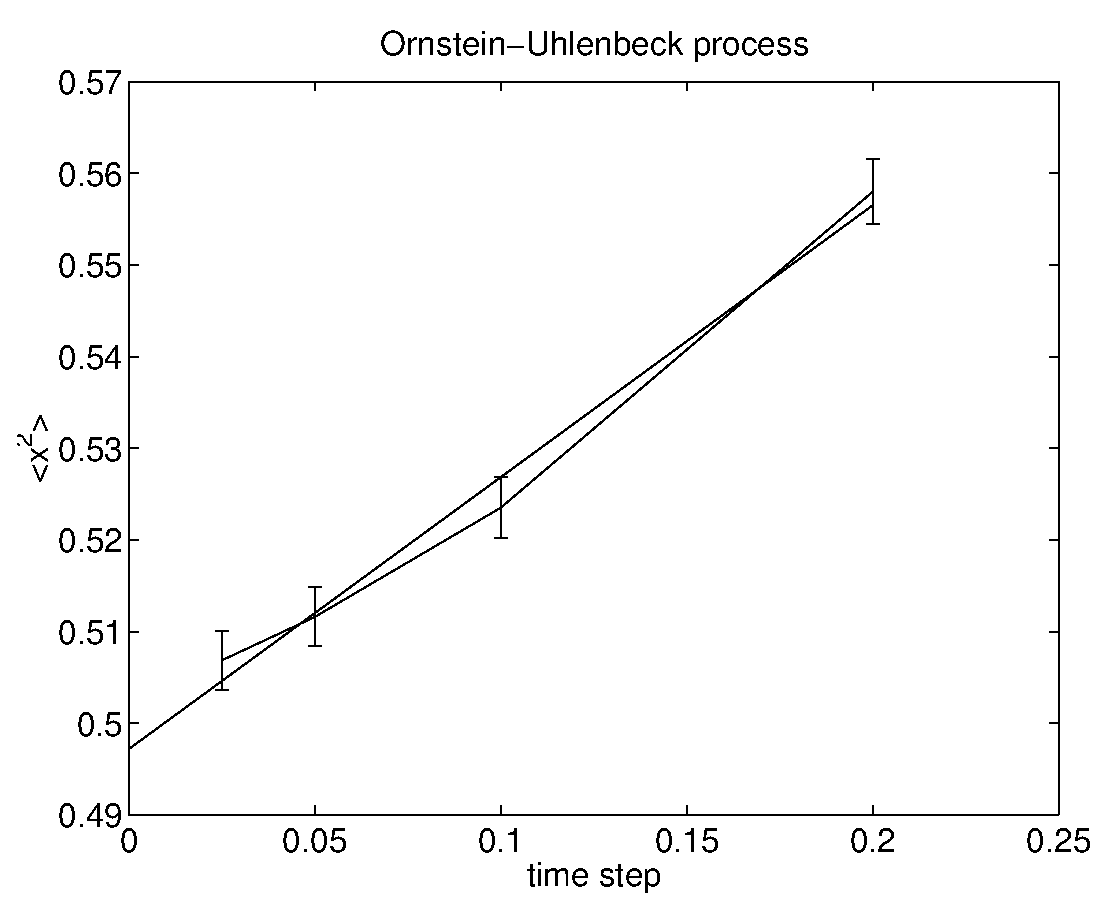
\includegraphics[width=10cm]{./Figures/f_sdeorn_50.eps}
\caption{Results of the simulation of the Ornstein--Uhlenbeck 
process with the stochastic Euler method for different values of 
the time step. The parameters of the Ornstein-Uhlenbeck process
are \texttt{q=1}, \texttt{D=1}. The simulation was run from
\texttt{tstart=0} to \texttt{tend=4} for 50000 realizations.
The timesteps used are \texttt{deltat=0.2, 0.1, 0.05, 0.025}.} 
\end{figure}
The figure clearly shows the expected linear convergence of the 
estimate to the expected exact result. The linear extrapolation 
leads to the estimate $<X^2>|_{t=4}=0.497182$, which is in very 
good agreement with the expected exact result. The simulation took
1729 sec on the laptop.

\subsection{Noise induced transitions}
In this second example of the application of the stochastic Euler 
method we want to simulate a stochastic differential equation with
multiplicative noise and consider noise induced transitions.

Let us begin by looking at the following deterministic dynamical 
system
\begin{equation*}
\frac{d}{dt} x(t) = \frac{1}{2} - x(t),
\end{equation*}
for $x \in [0,1]$. Obviously, this dynamical system has one 
fix point at $x_0=1/2$. This fix point can be shown to be 
asymptotically stable. 

We now want to perturb this system by adding a multiplicative 
noise term on the right hand of the above equation of motion.
To be precise we want to replace the deterministic equation of 
motion by the Ito stochastic differential equation
\begin{equation}
\label{SDENOISEIN}
dX(t) = (\frac{1}{2} - X(t))X(t)dt + \epsilon X(t) (1-X(t)) dW(t),
\end{equation}
where $\epsilon <0$

In order to understand the results of the simulation  we want to 
look at the stationary solution of the corresponding 
Fokker--Planck equation. The latter reads
\begin{equation*}
\frac{\partial}{\partial t} = - \frac{\partial}{\partial x} [a(X(t)) P(X,t) ]
      + \frac{1}{2} \frac{\partial^2}{\partial 
      x^2}[b(X(t))P(X,t)],
\end{equation*}
where we have used
\begin{equation*}
a(X(t)) = (\frac{1}{2} - X(t))X(t)
\end{equation*}
and
\begin{equation*}
b(X(t)) = [\epsilon x(t) (1-X(t))]^2.
\end{equation*}
Of course, the stationary solution has to satisfy
\begin{equation*}
\lim_{t \rightarrow \infty} \frac{\partial}{\partial t} P(X,t) =0
\end{equation*}
and hence
\begin{equation*}
\frac{d}{dx} [a(X(t)) P(X,t) ] - \frac{1}{2} \frac{\partial^2}{\partial 
      x^2}[b(X(t))P(X,t)] =0.
\end{equation*}
The above equation can be written as
\begin{equation}
\label{DDXJ}
\frac{d}{dx} J(x) =0,
\end{equation}
with 
\begin{equation*}
J(x) = a(X(t)) P(X,t)  - \frac{1}{2} \frac{\partial}{\partial 
      x}[b(X(t))P(X,t)].
\end{equation*}
In order to satisfy Eq. (\ref{DDXJ}) $J$ must be constant. If we 
assume that the stationary density $P_S(x) \longrightarrow 0$ for 
$|x| \longrightarrow \infty$ then the constant in question must be 
zero and we can conclude that
\begin{equation*}
\frac{d}{dx} [b(x) P_S(x)] = 2 a(X)P_S(x).
\end{equation*}
Dividing both sides by $b(x)P_S(x)$ we get
\begin{equation*}
\frac{d [b(x) P_S(x)]}{b(x) P_S(x)} = \frac{2a(x)}{b(x)}.
\end{equation*}
Integrating the above expression gives
\begin{equation*}
\ln [b(x) P_S(x)] = \int_c^x dx' \frac{2a(x')}{b(x')}
\end{equation*}
or
\begin{equation*}
P_S(x) = \frac{N}{b(x)} \exp{-\phi (x)},
\end{equation*}
where
\begin{equation*}
\phi(x) = - \int_c^x dx' \frac{2a(x')}{b(x')}.
\end{equation*}
The factor $N$ is a normalization constant to be chosen such that
\begin{equation*}
\int_a^b P_S(x) dx =1.
\end{equation*}

Transposing the above sketched general theory to the stochastic 
differential equation of interest  we get the stationary density,
which sometimes also called the invariant density,
\begin{equation*}
P_S(x) = \frac{N}{x(1-x)} \exp\left( - \frac{1}
           {\epsilon^2 x(1-x)}\right)
\end{equation*}

Now we are in the position to simulate the stochastic differential
equation (\ref{SDENOISEIN}). This will be done with the help of 
the program \texttt{sdenosein.m}.

\subsubsection{Listing of the program \texttt{sdenoisein.m}}
\inputlisting{./Listings/sdenoisein.m}
The program generates trajectories of the stochastic process with 
the help of the Euler algorithm. At the end of the simulation we evaluate 
numerically the stationary distribution with the help
of the MATLAB plotting function \texttt{hist}.

In a first run we perform a simulation of 5000 trajectories for 
the following parameters \texttt{xstart=0.5}, \texttt{epsilon=1},
\texttt{tend=4}, and \texttt{deltat=0.01}. The initial condition
was always chosen to be \texttt{xstart=0.5}. The resulting histogram
of the invariant density can be seen in Fig. 
(\ref{F_SDENOISEIN_1}).

\begin{figure}
\label{F_SDENOISEIN_1}
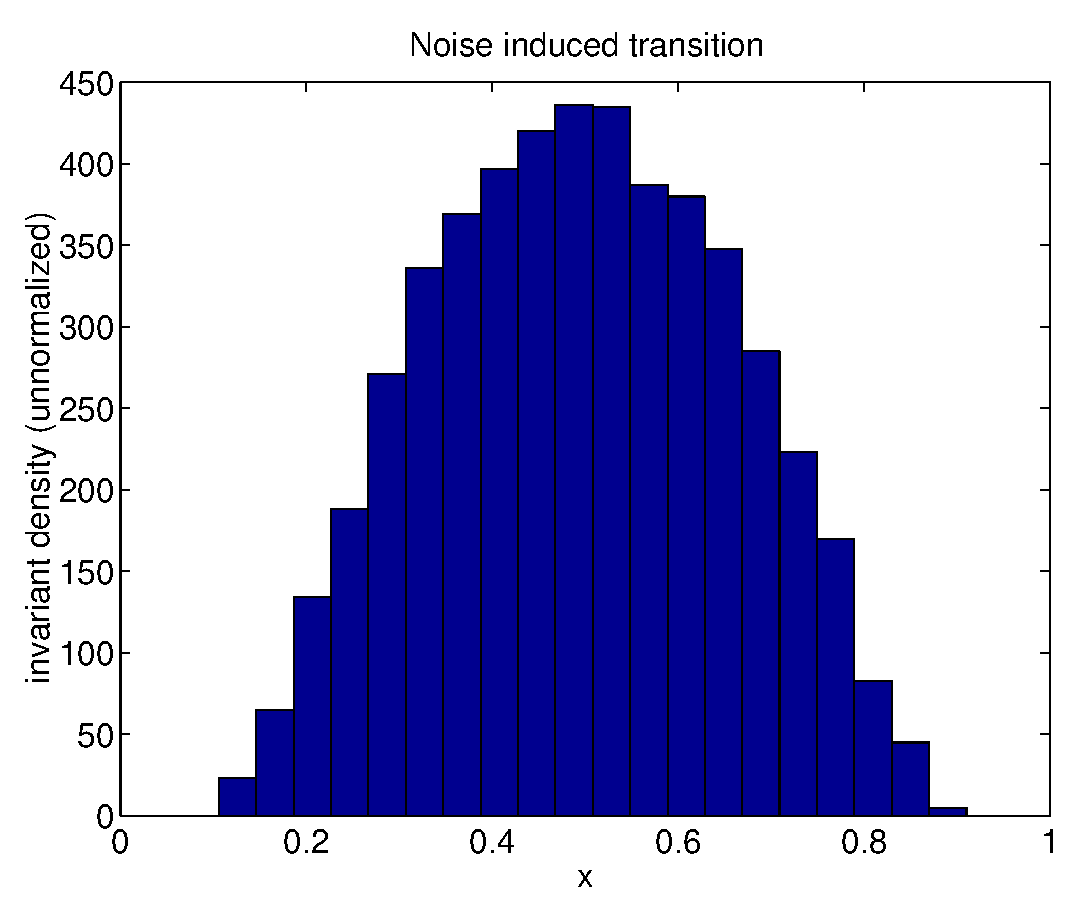
\includegraphics[width=10cm]{./Figures/f_sdenoisein_1.eps}
\caption{Histogram of the invariant density of the stochastic differential 
equation with multiolicative noise. The simulation was run from
\texttt{tstart=0} to \texttt{tend=4} for 5000 realizations.
The initial condition was chosen to be \texttt{xstart=0.5}.
The timestep used was \texttt{deltat=0.01} and the multiplicative noise 
constant was \texttt{epsilon=1}.} 
\end{figure}

It is clear from the histogram that the most probable value of $X$ 
lies around 0.5 and is therefore identical with the fixed point of 
the corresponding deterministic process.

Now we run the program with the same parameters as above but 
choose the multiplicative noise constant to be \texttt{epsilon=3}.
The result of this second simulation can be seen in Fig. 
(\ref{F_SDENOISEIN_2}).
\begin{figure}
\label{F_SDENOISEIN_2}
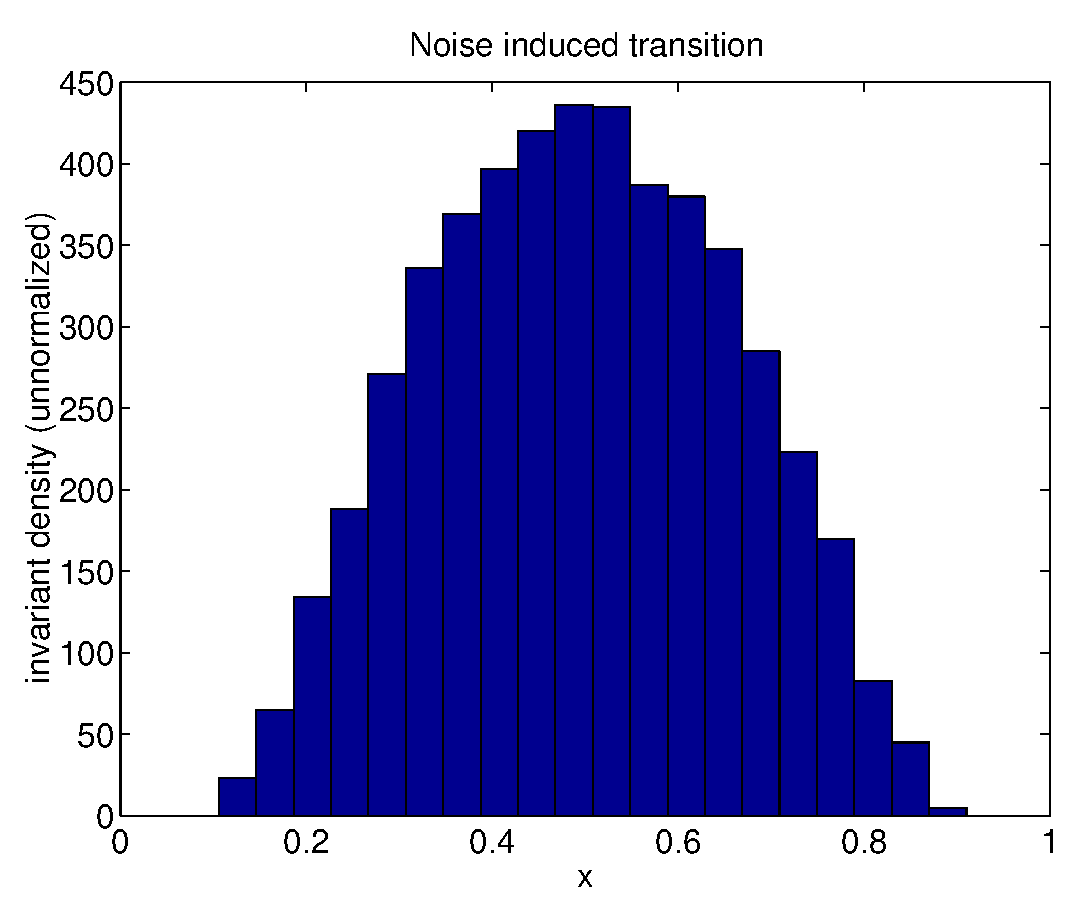
\includegraphics[width=10cm]{./Figures/f_sdenoisein_1.eps}
\caption{Histogram of the invariant density of the stochastic differential 
equation with multiolicative noise. The simulation was run from
\texttt{tstart=0} to \texttt{tend=4} for 5000 realizations.
The initial condition was chosen to be \texttt{xstart=0.5}.
The timestep used was \texttt{deltat=0.01} and the multiplicative noise 
constant was \texttt{epsilon=3}.} 
\end{figure}
It is evident from this figure that the invariant density changes 
its character. Now there is no longer one value of $X$ which is 
more probable. The histogram shows a minimum for $X=0.5$ and two 
equally high maxima at around 0.1 and 0.9. As a consequence of 
the larger noise the system undergoes a "stochastic bifurcation" 
which changes the number of the maxima of the invariant density. 
Such a phenomenon is called a {\em noise induced transition}.

Let us now try do see whether this observation is in agreement 
with the stationary density we have derived at the beginning of 
this subsection. The maxima of the stationary distribution are 
easily evaluated from the equation
\begin{equation*}
0 = \frac{d}{dx}P_S(x_m)
\end{equation*}
which explicitly reads
\begin{equation*}
0= (1-2x_m) [1- \epsilon^2 x_m (1-x_m) ].
\end{equation*}
For $0 < \epsilon <2$ the invariant density has an extremum, 
namley a maximum at $x_m =x_0= 1/2$, which is the fixed point of the 
deterministic equation of motion. For $\epsilon > 2$ the invariant
density posses a minimum at $x_0 =1/2$ and two maxima of equal 
height at $x_{m1,m2}$
\begin{equation*}
x_{m1,m2} = \frac{1}{2} \left(1 \pm  \sqrt{1 - (4/\epsilon^2)} 
\right).
\end{equation*}
Thus for the value of \texttt{epsilon=3} chosen in the second 
simulation the maxima are expected  to be at 0.8727 and 0.1273 
respectively. The histogram reproduced in Fig. (\ref{F_SDENOISEIN_2})
is in agreement with this theoretical prediction.


\section{Stochastic resonance}
In order to get aquainted with 
the numerical integration of stochastic differential equations we discuss a
phenomenon which occurs as
the response of a nonlinear system in the presence of noise: stochastic 
resonance. For a comprehensive introduction see \cite{Lanzara,Bulsara}. 
We already know that the effect of noise on the time evolution of 
deteministic linear system is rather trivial. If the statistical properties of
the input noise are known it is traightforward to compute the statistical
properties of the output signal. For nonlinear systems the situation changes
dramatically. The presence of the noise influences the evolution of the
system often in a counterintuitive way. The numerical integration of the
corresponding stochastic differential equations allows us to look at the
realizations of the process and to gain insight in these interesting
phenomena. 

The phenomenon of stochastic resonance was proposed by Benzi \textit{et al.}
\cite{Benzi,Benzi2} in a series of papers in which they address the problem
of the periodic switching of the Earth's climate between periods of relative
warmth and ice ages. It is known from the statistical analysis of continental
ice volume over the last million years that this switching is random and that 
it occurs with an approximate period of 100000 years. It is as well known that
the eccentricity of the Earth orbit varies with roughly the same period. 
However,
the associated variations of the solar energy influx on the earth surface are
so small, that climatologists doubt that  such a small external periodic force
effect might induce such climatic changes. In their seminal papers Benzi
\textit{et al.} represent the global climate with the help of a bistable
``climatic potential''. One minimum of the potential represents a small
temperture typical of an ice age, the other one a more  warm climate.
These authors then show that the weak periodic variation of the eccentricity
together with other random perturbations modelled as additive noise (e.g.
short--term climate fluctuations) might explain the periodicity observed for
the transition between one and the other of the two stable climate 
states. They name this
phenomenon stochastic resonance for the following reason: the
signal--to--noise ratio, i.e. the response of the system, is maximized when a
parameter of the stochastic force is tuned to an optimal value.

It is the aim of this section to introduce the basic principles of stochastic
resonance \cite{McNamara,Gammaitoni} and to simulate a simple model 
showing this phenomenon.
It is clear from the example discussed above that the basic mechanism  of 
stochastic resonance relies upon three essential ingredients:
a bistable system, a periodc driving signal, and a noise signal.

The simplest version of a one--dimensional nonlinear dynamical system 
is the damped anharmonic oscillator with the following equation of motion
\begin{equation}
m \frac{d^2x}{dt^2} + \gamma \frac{dx}{dt} = - \frac{dU(x)}{dx} 
 + \sqrt{D} \chi(t).
\end{equation}
The above Langevin equation describes the motion of a classical particle of
mass $m$ in a potential $U(x)$ and with an additive stochastic force
$\chi(t)$,
where $\chi(t)$
is a Gaussian white noise characteized by
\begin{equation}
\langle \chi(t) =0 \rangle; \;\;\; \langle \chi(t) \chi(t')\rangle =
\delta(t - t').
\end{equation}
The potential $U$ is bistable and we assume that it has the simple form
\begin{equation}
U(x) = -a \frac{x^2}{2} + b \frac{x^4}{4}.
\end{equation}
For $a> 0$ the potential $U$ is bistable with an unstable state at $x=0$
and two stable states at $x_s = \pm \sqrt{a/b}$. The stable states are
separated by a barrier of height $\Delta U = a^2/4b$. The system remains
dynamically stable for $b>0$, and becomes monostable for $a \le 0$.
Furthermore we assume that the system is overdamped by neglecting the inertial
term $m d^2x/dt^2$. 
Rescaling the resulting Langevin equation with the damping constant
$\gamma$  we finally obtain the so--called stochastic Ginzburg--Landau
equation
\begin{equation}
\label{Stoch_Ginzburg_Landau}
\frac{dx(t)}{dt} = ax - bx^3 + \sqrt{D} \chi(t),
\end{equation}
an equation which is often encountered in the theory of nonequilibrium
critical phenomena. 

\subsection{Reaction rate theory}
Let us now investigate some fundamental properties of the above dynamical
system. We begin by considering the case $D=0$ (no fluctuations). If the 
system is initially in a stable state it remains there for ever. 
The typical local
time scale is the relaxation time $\tau_r$ inside the wells. This time scale 
can be determined by considering small variations around the 
minimum of the well.
To do so we linearize Eq. (\ref{Stoch_Ginzburg_Landau}) 
around the stable state $x_s = \sqrt{a/b}$ with the help of
\begin{equation}
x(t) = x_s + \delta x(t)
\end{equation}
and obtain
\begin{equation}
\frac{d(\delta x)}{dt} = -2a \delta x.
\end{equation}
Thus, the  time scale $\tau_r$ of the relaxation inside the wells is
\begin{equation}
  \tau_r = \frac{1}{2a} = \frac{1}{U''(x_s)}.
\end{equation}

The situation changes in the presence of noise. The fluctuating forces allow
the system to jump between the two stable states. If the noise strength $D$ 
is small compared to the barrier height, these jumps are rare events. 
It is a well--know result of Kramers reaction--rate theory (see e.g.
\cite{Haenggi:Kramers}) that the mean escape time $T_e(x)$ out of one basin of
attraction can be written for sufficiently low noise ($\Delta U/D \gg 1$)in 
the form of the Arrhenius law
\begin{equation}
  \label{eq:Arrhenius}
  T_e(x) = A \exp(\Delta U(x)/D),
\end{equation}
where $A$ is a prefactor which depends on the form of the potential. For the
special potential we consider here, performing a Gaussian approximation of the
potentail around the minimum and the maximum and using the condition
$\Delta U/ D >> 1$ one gets the so--called Kramers
formula (or Arrhenius formula) for the escape time of a bistable system
\begin{equation}
\label{eq:Kramers}
  \tau_k = \frac{2\pi}{\sqrt{|U''(0)|U''(x_s)}} \exp [ 2 \Delta U / D ].
\end{equation}
The escape time $\tau_k$ is the global time scale of the bistable system.
The physical content of the assumptions we stated above is the following
one: The Kramers time $\tau_k$ is derived under the assumption that the
probability density within a well is roughly in equilibrium when the escape
takes place. Thus, the condition $\Delta U/D \gg 1$ guarantees that the two
time scales, the relaxation time and the Kramers time are different. The
system relaxes quickly (on a short time scale) to a local equilibrium at the
stable states and approaches global equilibrium (transitions over the barrier)
on a slow time scale. It follows from Eq. (\ref{eq:Kramers}) that
\begin{equation}
  \frac{\tau_k}{\tau_r} = 2 \sqrt{2} \pi \exp(2 \Delta U /D) \gg 1.
\end{equation}
The rate to jump over the barrier $W_k$ is obviously the inverse escape time
\begin{equation}
  w_k = \tau_k^{-1} = \frac{a}{\sqrt{2} \pi} \exp(-2 \Delta U/D).
\end{equation}

\subsection{The stochastic resonance}
Having reviewed some basilar results of the theory of nonlinear stochastic
systems we are now ready to look at the phenomenon of stochastic resonance.
In the preceeding subsections we made use only of two of the basic ingredients
of the recipe for stochastic resonance. The phenomenon only occurs in the
presence of a periodic driving signal. If we add such a signal to the bistable
system just considered its dynamics will be governed by the following Langevin
equation
\begin{equation}
  \frac{dx}{dt} = - \frac{\partial U(x,t)}{\partial x} + \sqrt{D} \chi(t), 
\end{equation}
where the bistable potential takes now the form
\begin{equation}
\label{eq:bistablepotential}
  U(x,t) = -a \frac{x^2}{2} +b \frac{x^4}{4} - Ax \cos(\omega_s t),
\end{equation}
where $A$ and $\omega_s= 2 \pi/T_s$ are the amplitude 
and the frequency of the periodic
signal. As a consequence of the periodic forcing term the potential tilts
periodically between up  and down. When the periodic force is at its
maximum (or minimum)  the difference between the escape rates from the two
states is maximum. The periodic forcing is assumed to be so
weak that it can not let the particle roll periodically from one potential
well into the other one. Nevertheless, the noise--induced hopping beween the
two wells  may become synchronized with the weak periodic forcing. This is 
signature of stochastic resonance. Stochastic resonace manifests itself by a
synchronization of activated hopping between the potential minima with the
weak periodic forcing. 

The manifestation of the phenomenon may be visualized with the help of the
output signal. It is clear that in the absence of the periodic driving
the escape process is induced by the fluctuating force and is random. Thus, in
this case the output signal $x(t)$ looks like dichotomous noise. The
probability density of residence times between two jumps is exponential
\begin{equation}
  P(t) = \frac{1}{\tau_k} \exp(-t/\tau_k),
\end{equation}
where the Kramers time can be
interpreted as the mean residence time spent by the system in one well.
The periodic driving force alters this situation. The modulation synchronizes
the hopping. The output signal reveals a quasiperiodic contribution to the
jump process, which has a maximum if the system jumps, on average, two times
per cycle of the external forcing. This is the stochastic resonance condition,
which for small driving frequencies $\omega_s \ll \omega_k$ 
can be approximated by \cite{Jung}
\begin{equation}
\label{eq:ResonanceCondition}
  T_s = 2 \tau_k = \frac{2 \pi \sqrt{2}}{a} \exp(2 \Delta U / D).
\end{equation}
The same condition formulated in terms of the noise intensity reads
\begin{equation}
\label{eq:ResonanceConditionD}
  D_0 = \frac{2 \Delta U}{\ln(a/(\sqrt{2} \omega_s)}.
\end{equation}
At this resonance condition the coherent contribution of the jump process has
a maximum.

Now that we have learned the basic aspects of stochastic resonance let us 
write a program to simulate it. Before doing so it is very helpful to write
the basic equations of motion in dimensionless form. To this end we write
the bistable potential (\ref{eq:bistablepotential}) in the form
\begin{equation}
  \label{eq:bistabledimless}
  U(x,t) = \Delta U \left[ -2\left( \frac{x}{x_s} \right)^2 
                           + \left( \frac{x}{x_s} \right)^4 \right] - 
                 U_1 \left(\frac{x}{x_s} \right) \cos(\omega_s t),.
\end{equation}
where $U_1 = A x_s$. The Langevin equation of motion can then be written as
\begin{equation}
  \label{eq:langevindimless1}
  \frac{dx}{dt} = 4 \Delta U \left( \frac{x}{x_s^2} - 
                   \frac{x^3}{x_s^4} \right)
                  + \frac{U_1}{x_s} \cos(\omega_s t)
                  + \sqrt{D} \xi(t).
\end{equation}
If we devide the above equation through $4 \Delta U$ and multiply it by $x_s$
\begin{equation}
  \label{eq:langevindimless2}
  \frac{1}{x_s} \frac{x_s^2}{4 \Delta U} \frac{dx}{dt} 
 =  \left( \frac{x}{x_s} - 
                   \frac{x^3}{x_s^3} \right)
                  + \frac{U_1}{ 4 \Delta U } \cos(\omega_s t)
                  + \frac{x_s}{4 \Delta U}\sqrt{D} \xi(t).
\end{equation}
If we now choose the unit of length to be $x_s$ and the time unit to be
$1/a$, note that $x_s^2/4 \Delta U = 1/a$, the dimensionless form of the above
equation reads
\begin{equation}
  \label{eq:langevindimless3}
  dx 
 =  \left( x - 
              x^3 \right)dt 
                  + \frac{U_1}{ 4 \Delta U} \cos(\omega_s t)dt
                  + \sqrt{D} \eta(t) \sqrt{dt},
\end{equation}
where for notational convenience we have named $x$ and $t$ to denote the 
corresponding dimensionless quantities and $D$ denotes the dimensionless
noise intensity. Recall, that in the units defined above $D$ has the dimension
$a x_s^2$.

HIER KOMMT DAS LISTING DES PROGRAMMES:

\verb|StochasticResonance.java|

Before running the program let us formulate the resonace condition in
dimensionless units. It follows from Eq. (\ref{eq:ResonanceConditionD}) that
\begin{equation}
  \label{eq:ResonanceConditionDless}
  D_0= \frac{1}{2 \ln (1/\sqrt{2} \omega_s)}.
\end{equation}
To give a numerical example, for $\omega_s= 0.1$ the  time scale matching
condition states that we have to choose $D= 0.2556$. Let us run now the
program keeping first $\omega_s$ fixed and varying $D$ and then keeping $D$
fixed and varying $\omega_s$.



Here comes the simulation and the discussion.


Now we could discuss:
\begin{itemize}
\item the periodic response
\item the signal to noise ratio
\end{itemize}

Let us finally look at the spectrum of the output signal. ...



Since its original formulation the phenomenon of stochastic resonance has been
observed in several physical and biological systems. These observations are
reviewed in 
\cite{Gammaitoni} and the introductory article \cite{Bulsara} .


%%%%%%%%%%%%%%%%%%%%%%%%%%%%%%%%%%%%%%%%%%%%%%%%%%%%%%%%%%%%%%%%%%

\section{Exercises}

\begin{Ex}
\label{Johnson_Noise}
\textbf{Johnson Noise \cite[]{gillespie:96} } \\
Johnson noise is the thermally generated electrical noise appearing in a conductor. 
Assume we have a rigid wire loop of self-inductance $L$ and resistance $R$ at
absolute temperature $T$. We can visualize this using the figure below. 
\begin{center}
\includegraphics[width=5cm]{f_johnson.eps}
\end{center}
There is no external potential, just the interactions between the conducting
electrons and the vibrations of the atomic lattice give rise to a temporally \text{var}ying
electromotive force in the loop (for details see \cite[]{gillespie:96}). 

The circuit equation gives (the integral of the electric potential around the 
loop must be zero)
$$ -RI(t)+V(t)-L\frac{dI(t)}{dt}=0.$$
Taking averages gives (assume $<V(t)>=0$) $$ -L\frac{d<I(t)>}{dt} =R<I(t)> .$$
If we can measure $I(t)$ we have an experimental way of determining $R$ and $L$.

We rewrite the first equation using $\tau:=L/R$ and $V(t):=Lc^{1/2}\Gamma(t)$, where
$\Gamma(t)$ is a Gaussian white noise and $c>0$ constant:
$$ \frac{dI(t)}{dt}=-\frac{1}{\tau}I(t)+c^{1/2}\Gamma(t) .$$
This is just the Langevin-equation for an Ornstein-Uhlenbeck process with
relaxation time $\tau$ and diffusion constant $c.$
The diffusion constant $c$ can be calculated by using the equipartition
theorem of statistical mechanics and applying the results for the 
Ornstein-Uhlenbeck process. We get $c=2kTR/L^2.$

Write a program to solve the Langevin equation for $I(t)$ with the initial
condition $I(t)=i_0.$ Use the Euler method for solving stochastic
differential equations. Use the three different sets of parameters:
\begin{itemize}
\item $\tau=1, c=1, i_0=0, \Delta t=0,001 $
\item $\tau=1, c=1, i_0=0, \Delta t=0,0001 $
\item $\tau=0,001, c=1.000.000, i_0=0, \Delta t=0,001 $
\end{itemize}
(Remark: the first and the third parameter set lead to the same
constant $\tau c^{1/2}$ for discussing $\tau\to 0$, the limit to Gaussian
white noise.)

The exact solution is ($\mathbf{N}( , )$ denotes a normal distribution):
$$ I(t)= \mathbf{N}\left(i_0e^{- \frac{R}{L}(t-t_0)} , \frac{kT}{L}
        \left(1-e^{-2\frac{R}{L}(t-t_0)}\right) \right) .$$

Also calculate the (auto-)covariance function $ C_I(t'):=\text{cov}(I_s(t),I_s(t+t')) $
(the subscript $s$ indicates that the process should be stationary)
and analyze the spectrum thereof - use a log-log plot for the
spectrum. The spectrum is the cosine transform of $C_I$.
\end{Ex}


%%%%%%%%%%%%%%%%%%%%%%%%%%%%%%%%%%%%%%%%%%%%%%%%%%%%%%%%%%%%%%%%%%%%%

\bibliographystyle{peter}
\bibliography{V_98,simulit}



%%% Local Variables: 
%%% mode: latex
%%% TeX-master: t
%%% End: 
